To solve this problem I need to give you a few definitions.

If is \(n\) an integer and is a \(p\) prime factor of \(n\), the multiplicity of \(p\) in \(n\) is defined as the number of times \(p\) can divide \(n\). For example, the multiplicity of $2$ in $24$ is $3$ since you can divide $24$ up to three times, and no more. Let's denote the multiplicity of $p$ in $n$ by $o_p(n)$. For example \(o_2(24) = 3\), 

Then I need you to compute the function $f(n)$ defined as:

$$f(n) = \prod_{\substack{p \\ p \geq 2 \text{ is a prime dividing } n}} p^{o_p(n)}$$

Then I need you to compute the number $k$ defined as:

\[\int_{0}^{2\sqrt{5}} x \, dx\]

Finally, I will give you one number $n$ and you will have to generate $f(n)$ numbers from $1$ to $k$ inclusive. If you followed the same process as I did when generating the test data, you should get the same results.

\large{\bf{Bounds:}}
$$ 1 \le n \le 10 $$

This is how you make LaTeX stuff:

This is 100\% worth \$\$\$ bills.

This is \textbf{bold} text. So \bf{brave}.

This is \textit{italic} text. So \it{italian}.

This is \texttt{monospace} text. So \tt{typewriter-y}.

This is \underline{underlined} text. So \emph{emphasized}.

This is \sout{strikethrough'ed} text.

This is \textsc{uppercase} text.

Here are all the font sizes.

\tiny{tiny} or \scriptsize{scriptsize}

\small{small}

\normalsize{normalsize}

\large{large}

\Large{Large}

\LARGE{LARGE}

\huge{huge}

\Huge{Huge}

\HUGE{HUGE}

Here is a link \url{http://example.com}

Here is a nicer \href{http://example.com}{link}

You can also nest all of these together. \href{http://example.com}{\HUGE{\sout{\tt{\bf\it{{link}}}}}}

Here is a picture for your troubles 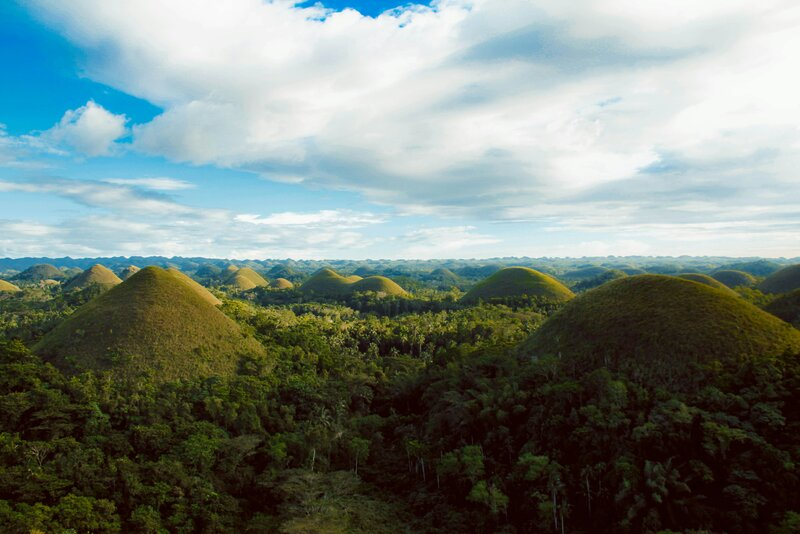
\includegraphics{/tasks/crazy-problem/attachments/path/to/chocolate-hills.jpg}
